\documentclass{article}
\usepackage[utf8]{inputenc}
\usepackage{graphicx}
\usepackage{hyperref}

\makeatletter
\def\maxwidth{\ifdim\Gin@nat@width>\linewidth\linewidth\else\Gin@nat@width\fi}
\def\maxheight{\ifdim\Gin@nat@height>\textheight\textheight\else\Gin@nat@height\fi}
\makeatother

% Scale images if necessary, so that they will not overflow the page margins by
% default, and it is still possible to overwrite the defaults using explicit
% options in \includegraphics[width, height, ...]{}
\setkeys{Gin}{width=\maxwidth,height=\maxheight,keepaspectratio}
\setlength{\parindent}{0pt} \setlength{\parskip}{6pt plus 2pt minus 1pt}
\setlength{\emergencystretch}{3em}  % prevent overfull lines
\providecommand{\tightlist}{%
\setlength{\itemsep}{0pt}\setlength{\parskip}{0pt}} \setcounter{secnumdepth}{0}

\title{\href{http://www.newstatesman.com/lifestyle/2014/04/kimberl-crenshaw-intersectionality-i-wanted-come-everyday-metaphor-anyone-could}{Kimberl\'{e} Crenshaw on intersectionality: ``I wanted to come up with an everyday metaphor that anyone could use''}}
\author{Bin Adewunmi}
\date{2 April 2014}

\begin{document}
\maketitle

Kimberl\'{e} Crenshaw's ears must have been burning with alarming regularity
and intensity over the last couple of years. We meet in one of the dining rooms
of her hotel in central London, her base while she's on a whistlestop lecture
tour. Two days before our meeting she spoke at the School of Oriental and
African Studies, and later this evening, she will speak at the London School of
Economics. Her subject is intersectionality and feminism. In recent times,
intersectionality theory --- the study of how different power structures
interact in the lives of minorities, specifically black women, a theory she
named in the 1980s --- has enjoyed a resurgence in popular and academic
feminism. Her name and her work has become an introductory point for feminists
of all stripes.

Of course, she says, the concept of intersectionality is not exactly new. ``So
many of the antecedents to it are as old as Anna Julia Cooper, and Maria
Stewart in the 19th century in the US, all the way through Angela Davis and
Deborah King,'' she says. ``In every generation and in every intellectual
sphere and in every political moment, there have been African American women
who have articulated the need to think and talk about race through a lens that
looks at gender, or think and talk about feminism through a lens that looks at
race. So this is in continuity with that.''

\begin{figure}[h]
	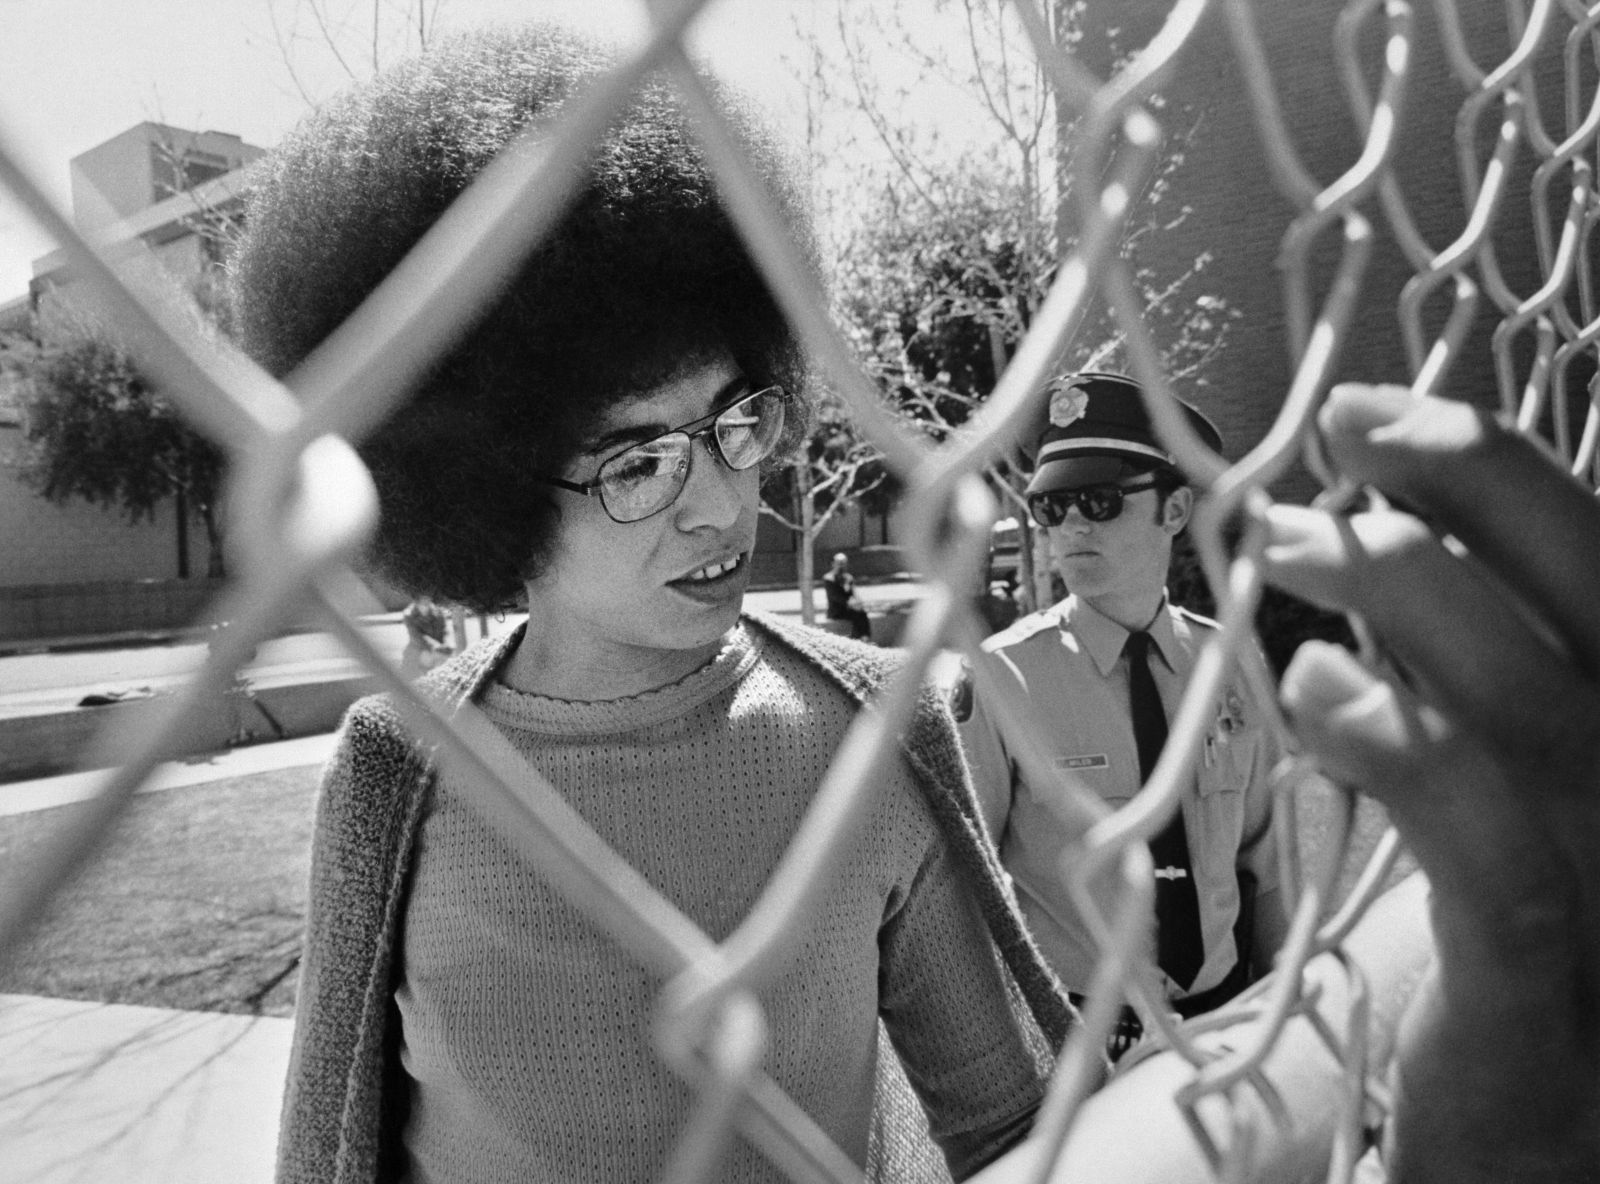
\includegraphics{.resources/Getty72.jpg}
	\caption{Angela Davis arrives at court in 1972. Photo: Getty}
\end{figure}

For Crenshaw, a law professor at UCLA and Columbia, intersectionality theory
came about specifically to address a particular problem. ``It's important to
clarify that the term was used to capture the applicability of black feminism
to anti-discrimination law,'' she says. In
\href{http://www.lse.ac.uk/newsAndMedia/videoAndAudio/channels/publicLecturesAndEvents/player.aspx?id=2360}{the
	lecture she delivered at the LSE later that evening}, she brought up the
case of Degraffenreid vs General Motors, in which five black women sued GM on
the grounds of race and gender discrimination. ``The particular challenge in
the law was one that was grounded in the fact that anti-discrimination law
looks at race and gender separately,'' she says. ``The consequence of that is
when African American women or any other women of colour experience either
compound or overlapping discrimination, the law initially just was not there to
come to their defence.''

The courts' thinking was that black women could not prove gender discrimination
because not all women were discriminated against, and they couldn't prove race
discrimination because not all black people were discriminated against. A
compound discrimination suit would, in the courts' eyes, constitute
preferential treatment, something nobody else could do. Crenshaw laughs when
she adds: ``Of course, no one else had to do that. Intersectionality was a way
of addressing what it was that the courts weren't seeing.''

Cases like these informed much of her earlier work on intersectionality ---
trying to show how these African American plaintiffs' arguments rested on the
ability to show that the discrimination they were experiencing was the
combination of two different kinds of policies. But there was an additional
point to the theory as well: pointing out that the tools being used to remedy
the overlapping discrimination --- anti-discrimination law --- were themselves
inadequate. ``You've got to show that the kind of discrimination people have
conceptualised is limited because they stop their thinking when the
discrimination encounters another kind of discrimination,'' she says. ``I
wanted to come up with a common everyday metaphor that people could use to say:
``it's well and good for me to understand the kind of discriminations that
occur along this avenue, along this axis --- but what happens when it flows
into another axis, another avenue?''

Laid out like this, it may seem baffling that so many have had a problem with
the idea of intersectionality. What is it, I asked Crenshaw, that makes it so
difficult for people to grasp? She pauses briefly before she answers. ``I'm
only speculating, but there lots of different reasons. I mean,
intersectionality is not easy,'' she says. ``It's not as though the existing
frameworks that we have --- from our culture, our politics or our law ---
automatically lead people to being conversant and literate in
intersectionality.''

On the charge that intersectionality is not new, she gets philosophical.
``Well, a lot of things aren't new,'' she says. ``Class is not new and race is
not new.  And we still continue to contest and talk about it, so what's so
unusual about intersectionality not being new and therefore that's not a reason
to talk about it? Intersectionality draws attention to invisibilities that
exist in feminism, in anti-racism, in class politics, so obviously it takes a
lot of work to consistently challenge ourselves to be attentive to aspects of
power that we don't ourselves experience.''  But, she stresses, this has been
the project of black feminism since its very inception: drawing attention to
the erasures, to the ways that ``women of colour are invisible in plain
sight''.

``Within any power system,'' she continues, ``there is always a moment --- and
sometimes it lasts a century --- of resistance to the implications of that. So
we shouldn't really be surprised about it.''

There is sometimes a failure to make analogies, she says. Feminists who have
answers for the questions of class politics and how it plays out along gender
lines sometimes exhibit an unwillingness to apply the same principles around
feminism and race. ``That ability to be intersectional --- even though it's not
called that --- isn't replicated in [this] conversation,'' she says. ``I think
that the same kind of openness and fluidity and willingness to interrogate
power that we as feminists expect from men in alliance on questions of class
should also be the expectation that women of colour can rely upon with our
white feminist allies.''

I bring up a tweet I recently read, about the ``perils of yelling at white
women for a living'' to ask what form pushback takes when discussing
intersectionality in feminism. ``At the end of the day, it really is a question
of power: who has the power to end the debate? To walk away? To say, `I'm done
talking about it, and I can go on with my rhetoric in a ``business as usual''
kind of response?''' She smiles. ``Sometimes it feels like those in power frame
themselves as being tremendously disempowered by critique. A critique of one's
voice isn't taking it away. If the underlying assumption behind the category
`women' or `feminist' is that we are a coalition then there have to be
coalitional practices and some form of accountability.''

But she also stresses the importance of black feminists being the originators
of dialogues about their own experience. ``When I was writing in the late 80s,
there was a strain of discourse among women who were not the subjects of
traditional feminism, to simply make critique a difference,'' she says. ``So
just the claim of `woman' or `feminist', prompted some women of colour to say,
`but that's not me'. Well, yeah --- that might not be you. But say what
difference it makes that it's not you --- what difference does it make in what
kinds of interventions come out of a feminist frame that doesn't attend to
race?'' She pauses, spreads her hands. ``That is our responsibility. It's up to
us. Granted, the space has to be open and there has to be a sense of
receptivity among the sisterhood, but I really don't want other women to feel
that it's their responsibility to theorise what's happening to us. It's up to
us to consistently tell those stories, articulate what difference the
difference makes, so it's incorporated within feminism and within anti-racism.
I think it's important that we do that apart, because we don't want to be
susceptible to the idea that this is just about the politics of recognition.''

No discussion of Crenshaw's work can be complete without discussing the
congressional hearings of October 1991, organised to address the claim that
\href{http://en.wikipedia.org/wiki/Clarence_Thomas}{Supreme Court nominee
	Clarence Thomas} had sexually harassed a colleague, Anita Hill. In his
denial of the allegations, Thomas said it was a ``high tech lynching''.
Crenshaw was part of the legal team that represented Hill --- and arguably
changed the course of history with regards to the recognition of sexual
harassment in the workplace. A documentary film, Anita, has been made of the
events of the time, a period Crenshaw describes as ``life-defining''.

\begin{figure}[h]
	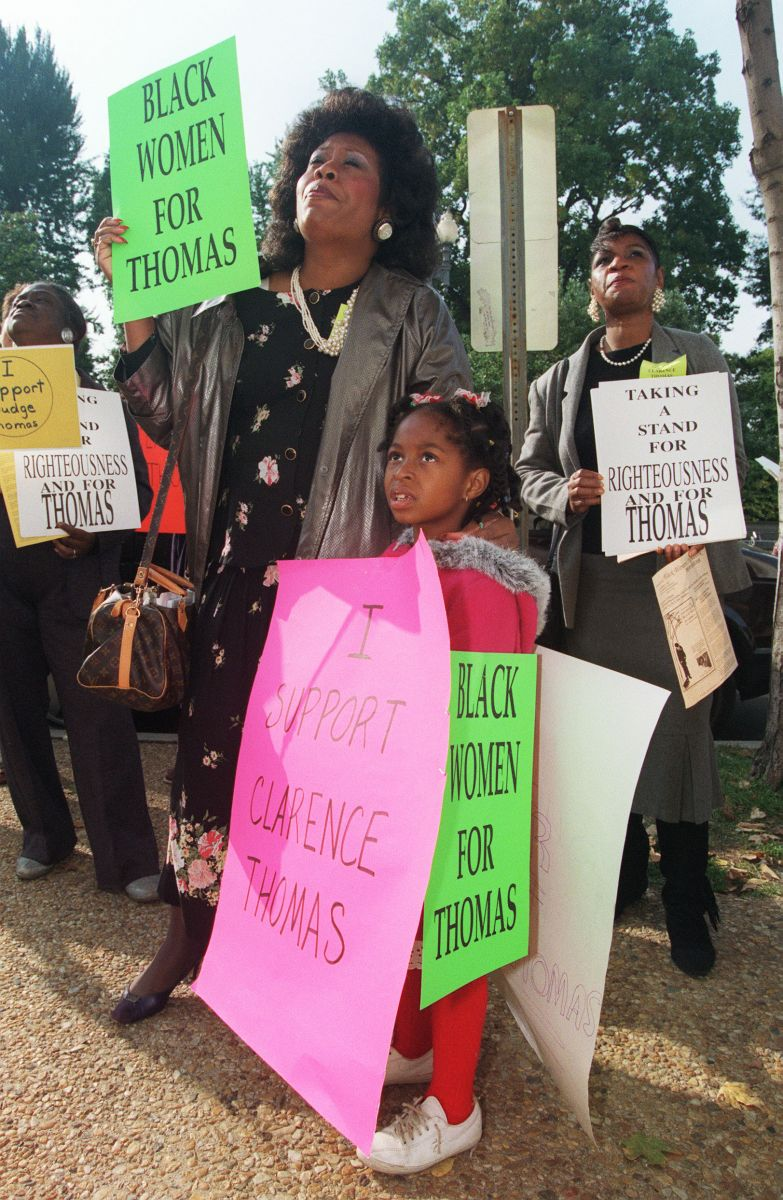
\includegraphics{.resources/Getty91.jpg}
	\caption{Pro-Clarence Thomas demonstrators in 1991. Photo: Getty}
\end{figure}

``When we were defending Anita Hill, it was it felt like there was 10 of us
against the whole world,'' she says. ``There was overwhelming criticism of
Anita Hill from Clarence Thomas's camp, the Republican camp, from the White
House, from the senate judiciary committee. And the Democrats were not
defending her.'' Thomas's ``lynching'' comment, she says, communicated to many
African Americans this was a race issue --- leaving Hill with no base to rally.
``Lynching is representative of the quintessential moment of racism --- and
that in turn centres African American male experiences,'' she says.

Crenshaw talks about a sort of ``collective forgetting'' --- the fact that
black women were not spared from lynching themselves, and the way that racist
sexism played out for black women involved sexual violence that was never
prosecuted.  Rosa Parks, she says, ``was a rape crisis advocate before she sat
down on that Montgomery bus. The very fact that there are a range of
experiences around sexualised racism that's not remembered --- and we only
remember one experience - is what then replayed itself in the 1990s.''

\href{http://www.thenation.com/article/163814/black-women-still-defense-ourselves}{She
	describes coming out of the Capitol} to find it ringed by largely African
American women ``holding hands singing gospel songs in support of Clarence
Thomas. It was like one of these moments where you literally feel that you have
been kicked out of your community, all because you are trying to introduce and
talk about the way that African American women have experienced sexual
harassment and violence. It was a defining moment.''

One consequence of this was Anita Hill's claim being taken up by mainstream
white feminists --- only she was stripped of her race, reinforcing the idea
that the case was a race vs. gender issue. ``She simply became a colourless
woman, and we as African American women feminists were trying to say, `you
cannot talk about this just in gender terms --- you have to be intersectional
--- there is a long history you cannot ignore,' but they didn't have the skills
to be able to talk about it,'' she says. That led to another big moment: the
moment when, as Crenshaw puts it, African American feminists had to ``buy their
way into the conversation''.

Nearly 2,000 African American feminists across the US collectively raised
\$60,000 and bought ad space in the New York Times. The ad, called African
American Women in Defense of Ourselves, was signed by 1,600 women, and covered
among other things, the historical discrimination against black women, as well
as what had been happening in the hearings. ``That was a moment where black
women came forward. Twenty years later,'' says Crenshaw, ``that has been
forgotten.'' The legacy of the Anita Hill case is one that subsequent
generations of women in the workplace will benefit from. ``Many women who talk
about the Anita Hill thing, they celebrate what's happened with women in
general: the fact that we have more elected officials now because they were
outraged when they saw what the men were doing, Emily's List came in and really
helped women get elected, and so on. So sexual harassment is now recognised;
what's not doing as well is the recognition of black women's unique experiences
with discrimination.''

The forgetting is important to note. Crenshaw recalls the strong
anti-harassment work of the civil rights movement, and speaks of a ``certain
ahistoricism'' in some of the conversations around feminism and anti-racism
work.. ``Intersectionality was something I wrote in 1986, '87 and there's whole
generation now that has come to the conversation after black feminism and other
forms of intersectional work tilled the soil,'' she says. ``And I think
sometimes its hard for people to imagine what the world was like at the point
when none of that work had been done. So I think it's useful to tell
genealogies that include social histories --- so people have a sense that the
way we talked about it then was as against the constraints of the time. And the
way way we talk about it now has built upon that. There are many things that
are forgotten, and many other things that are elevated.''

\end{document}
